\subsection{一元积分不等式}

	\begin{ti}
		已知函数 $f(x)$ 在区间 $[a,b]$ 上连续并单调增加,求证:
		\[
			\int_{a}^{b} \Biggl( \frac{b - x}{b - a} \Biggr)^{n} f(x) \dd{x} \leq \frac{1}{n + 1} \int_{a}^{b} f(x) \dd{x} (n \in \mathbb N).
		\]
	\end{ti}

	\begin{ti}
		设 $f(x)$ 在 $[a,b]$ 上连续,且 $f(x) > 0$,证明:
		\[
			\ln \left[ \frac{1}{b - a} \int_{a}^{b} f(x) \dd{x} \right] \geq \frac{1}{b - a} \int_{a}^{b} \ln f(x) \dd{x}.
		\]
	\end{ti}

	\begin{ti}
		设 $f(x)$ 二阶可导,$f''(x) \geq 0$,$g(x)$ 为连续函数,若 $a > 0$,求证:
		\[
			\frac{1}{a} \int_{0}^{a} f\bigl[g(x)\bigr] \dd{x} \geq f\left[ \frac{1}{a} \int_{0}^{a} g(x) \dd{x} \right].
		\]
	\end{ti}

	\begin{ti}
		设 $f(x)$ 在闭区间 $[0,1]$ 上有二阶导数,且 $f\bigl( \frac{1}{2} \bigr) = 1$,$f''(x) > 0$,证明 $\int_{0}^{1} f(x) \dd{x} \geq 1$.
	\end{ti}

	\begin{ti}
		\begin{enumerate}
			\item 证明不等式
			\[
				\ln(n+1) < 1 + \frac{1}{2} + \frac{1}{3} + \cdots + \frac{1}{n} < 1 + \ln n;
			\]
			\item 证明数列 $a_{n} = 1 + \frac{1}{2} + \frac{1}{3} + \cdots + \frac{1}{n} - \ln(n+1)$ 单调增加,且 $0 < a_{n} < 1$.
		\end{enumerate}
	\end{ti}

	\begin{ti}
		当 $x \geq 0$ 时,在曲线 $y = \ee^{-2x}$ 上面作一个台阶曲线,台阶的宽度皆为 $1$(如图~\ref{fig:1.3.5}). 求图中无穷多个阴影部分的面积之和 $S$.
		\begin{figure}[htbp]
			\centering
			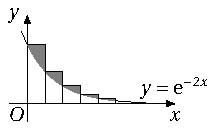
\includegraphics[scale=1]{figure/fig1-3-5.pdf}
			\caption{}\label{fig:1.3.5}
		\end{figure}
	\end{ti}

	\begin{ti}
		求极限 $\lim_{n \to \infty} \frac{\sum_{k=1}^{n} \frac{1}{k}}{\ln n}$.
	\end{ti}